\subsubsection*{Add.2}
\subsubsection*{(a)}
\paragraph{}
From Figure 2. The optimal $\gamma$ is 0.35 and the corresponding objective value is 0.4809.
\begin{figure}[h]
	\centering
	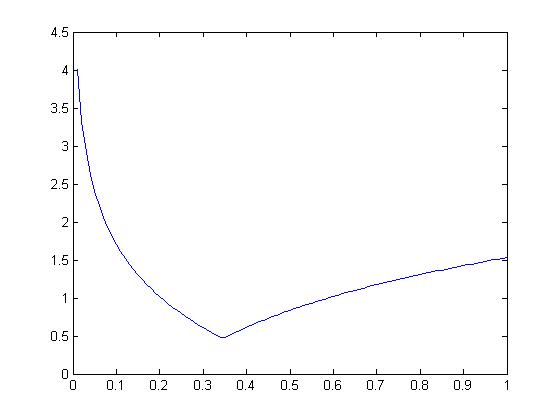
\includegraphics[scale=0.5]{equalpower}
	\caption{Equal Lamp Power}
\end{figure}
\subsubsection*{(b)}
\paragraph{}
$x = [1\ 0\ 1\ 0\ 0\ 1\ 0\ 1\ 0\ 1]^T$ and $p=0.8628$.
\subsubsection*{(c)}
\paragraph{}
$\rho =0.2200$,  $x = [0.5\ 0.4773\ 0.0832\ 0\ 0.4559\ 0.4353\ 0.4595\ 0.4306\ 0.4035\ 0.4525]^T$ and $p=0.4440$.
\subsubsection*{(d)}
\paragraph{}
With cvx we acquired a solution $x=[1\ 0.1165\ 0\ 0\ 1\ 0\ 1\ 0.0249\ 0\ 1]^T$ and an objective value $p=0.4198$.
 
\subsubsection*{(e)}
\paragraph{}
With cvx we acquired a solution $x=[1\ 0.1896\ 0\ 0\ 1\ 0\ 1\ 0.1640\ 0\ 1]^T$ and an objective value $p=0.3664$.
\subsubsection*{(f)}
\paragraph{}
With cvx we acquired the exact solution as $x=[1\ 0.2023\ 0\ 0\ 1\ 0\ 1\ 0.1882\ 0\ 1]^T$ and objective value $p=0.3575$. 
